\documentclass[fleqn, 10pt]{article}

% Paquetes necesarios
\usepackage[utf8]{inputenc}
\usepackage{graphicx} 
\usepackage{amsthm, amsmath}
\usepackage{nccmath} %Para centrar ecuaciones
\usepackage{graphicx}
\usepackage{enumitem}

% Personalizo mi alfabeto
\DeclareMathAlphabet{\pazocal}{OMS}{zplm}{m}{n}
\newcommand{\Lb}{\pazocal{L}}

% Definimos los entornos para definiciones, teoremas, etc...
\theoremstyle{plain}
\newtheorem{proposicion}{Proposición}

\theoremstyle{definition}
\newtheorem{definition}{Definición}[section]
\newtheorem{example}{Ejemplo}[section]

%Definimos el título
\title{Teoría de Autómatas y Lenguajes Formales\\[.4\baselineskip]Práctica 4}
\author{José Manuel Rodríguez Chicano}
\date{\today}

%Comienzo del documento
\begin{document}

%Generamos el título
\maketitle

\section{Ejercicio 1}

Create the simplest WHILE program that computes the diverge function (with
zero arguments) and compute the codification of its code.
\\
\\
La forma más fácil de realizar un programa WHILE sin argumentos de entrada que compute una divergencia es aquel cuyo bucle nunca llegue a 0 y la condición para que este termine sea cuando una variable X llegue a 0.
\begin{center}
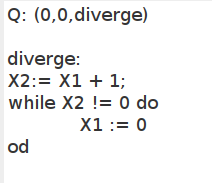
\includegraphics[width=10cm, height=10cm]{2.png}
\end{center}
Y la computación de su código realizado en el octave con la función CODE2N sería la siguiente:


\begin{center}
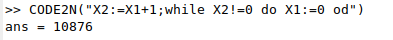
\includegraphics[width=10cm, height=2cm]{1.png}
\end{center}

\section{Ejercicio 2}

Create an Octave script that enumerates all the vectors.
\\

Al ser posible establecer una biyección de $N$ con el conjunto de vectores $N^*$. Se puede crear un programa que imprima los N vectores por pantalla.


\begin{center}
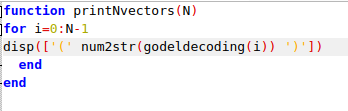
\includegraphics[width=5cm, height=2cm]{3.png}
\end{center}

Y podemos comprobar su funcionamiento con el propio OCTAVE ejecutando el código con una N cualquiera en este caso 40.


\begin{center}
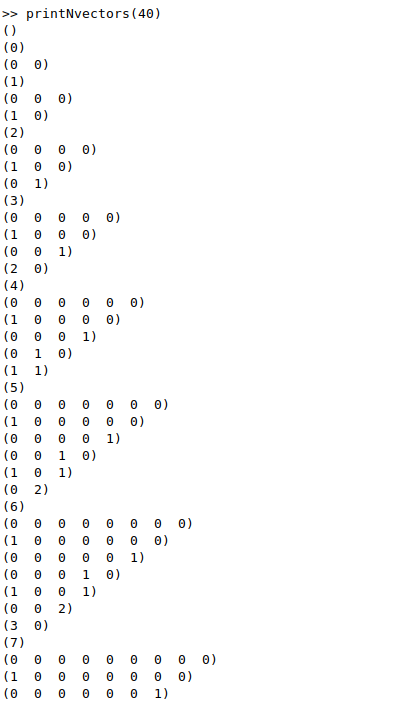
\includegraphics[width=5cm, height=9cm]{4.png}
\end{center}

\section{Ejercicio 3}
Create an Octave script that enumerates all the WHILE programs.
\\
\\
Los programas WHILE también pueden establecer una biyección con el conjunto $N$
\\ 
\\
Así podemos crear un código que imprima en pantalla los N primeros programas WHILE asociados a cada número natural de la siguiente manera:


\begin{center}
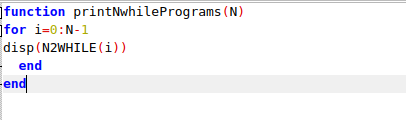
\includegraphics[width=10cm, height=6cm]{6.png}
\end{center}

Y usando OCTAVE podemos comprobar el funcionamiento del mismo:
\begin{center}
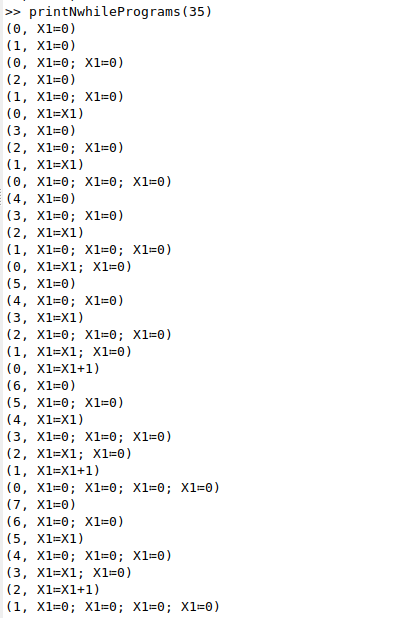
\includegraphics[width=5cm, height=7cm]{5.png}
\end{center}

\end{document}